% !TEX root = lectnote.tex
% !TEX spellcheck = en_GB-oed 

\chapter{Proof techniques}\label{cha:proof}

\section{Proofs by induction}
In mathematics one often uses induction to prove general statements. Let us see how this argument works.
Suppose we have a statement $S(n)$ which depends on $n$. When we apply induction we prove that $S(n_0)$
is true for the smallest possible value $n_0$. Then we show that if the statement is true for all possible values
less than $n$, then the statement is also true for $n$. Finally, we conclude that the statement is true for all $n\geq n_0$.
There is a very similar notion called recursion. For example we can define $n!$ as follows
\begin{equation*}
n!=
\begin{cases}
1 & \mbox{ if }n=1,\\
n\cdot(n-1)! & \mbox{ if }n>1.
\end{cases}
\end{equation*}
The basic idea is that we can compute e.g.\ $100!$ if we have computed $99!$, $98!$, $\ldots$, $1!$. Induction works in the same way,
if we can prove a statement for certain smaller instances, then we can prove it for large values as well. More about recursion
will follow in Chapter~\ref{Recurrence sequences}. 

Now we study induction in more detail.
\begin{theorem}[Mathematical Induction I]
Let $S(n)$ be a statement depending on $n\in\mathbb{N}$. Suppose that 
\begin{enumerate}
\item[(a)] $S(1)$ is true,
\item[(b)] if $S(k)$ is true for some $k\in\mathbb{N}$, then $S(k+1)$ is true.
\end{enumerate}
Then $S(n)$ is true for all $n\in\mathbb{N}$.
\end{theorem}
\begin{proof}
Suppose that the statement $S(n)$ is false for some $n\geq 1$. Denote by $m$ the smallest such value.
We have that $m>1$, since by part $(a)$ we know that $S(1)$ is true. Since $m$ is as small as possible, $S(k)$ is true for $1\leq k < m$.
As a special case we have that $S(m-1)$ is true. From part $(a)$ and $(b)$ one obtains that the statement is true for $S(m-1+1)=S(m)$.
Thus the assumption that $S(n)$ is false for same $n\geq 1$ is false.
\end{proof}
Let us consider a simple example. Let $S(n)$ be the statement that 7 divides $8^n-1$. First we do some numerical experiments
\begin{center}
\begin{tabular}{|c|c|}
\hline
$n$ & $8^n-1$\\
\hline
1 & $7=1\cdot 7$\\
\hline
2 & $63=9\cdot 7$\\
\hline
3 & $511=73\cdot 7$ \\
\hline
\end{tabular}
\end{center}
that is, the statement is true for $n\in\halmaz{1,2,3}$. Hence part $(a)$ of the theorem is fulfilled. Assume that $S(k)$ is true for some
$k\in\mathbb{N}$. It remains to be proved that $S(k+1)$ is true. We have that $S(k)$ is true, that is, 7 divides $8^k-1$. Hence there exists
an integer $A$ such that $8^k-1=7\cdot A$. We would like to prove that $8^{k+1}-1$ is a multiple of 7 as well. We try to express $8^{k+1}-1$
using $8^k-1$. A natural idea is to multiply the equation $8^k-1=7\cdot A$ by 8:
$$
8(8^k-1)=7\cdot A\cdot 8,
$$
that is, 
$$
8^{k+1}-8=7\cdot A\cdot 8.
$$
Now we add 7 to obtain the right form on the left-hand side:
$$
8^{k+1}-1=7\cdot A\cdot 8+7=7(8A+1).
$$
It means that $S(k+1)$ is true since we got that $8^{k+1}-1$ is divisible by 7.

Another area where induction can often be applied is proving mathematical identities. Now we prove that the sum of the first $n$ positive 
integers is $\frac{n(n+1)}{2}$. Let us compute the sum of the first $n$ integers for $n\in\halmaz{1,2,3,4,5}$
\begin{center}
\begin{tabular}{|c|c|}
\hline
$n$ & $\sum_{i=1}^n i$\\
\hline
1 & $1=\frac{1\cdot 2}{2}$\\
\hline
2 & $1+2=\frac{2\cdot 3}{2}$\\
\hline
3 & $1+2+3=\frac{3\cdot 4}{2}$\\
\hline
4 & $1+2+3+4=\frac{4\cdot 5}{2}$\\
\hline
5 & $1+2+3+4+5=\frac{5\cdot 6}{2}$\\
\hline
\end{tabular}
\end{center}
So it seems that the formula is correct. However, we have not proved the statement, we only checked that the statement is correct for $n\in\halmaz{1,2,3,4,5}$.
Here $S(n)$ is the statement that the sum of the first $n$ positive integers is $\frac{n(n+1)}{2}$. We have that $S(1)$ is true. Assume that $S(k)$ is true
for some $k\geq 1$, that is, 
$$
\sum_{i=1}^k i=\frac{k(k+1)}{2}.
$$
We have to prove that $S(k+1)$ is true. That is, we have to consider the sum of the first $k+1$ integers, which is
$$
\sum_{i=1}^{k+1} i =1+2+\ldots+k+(k+1)=(1+2+\ldots+k)+(k+1).
$$
By the induction hypothesis 
$$
1+2+\ldots+k=\frac{k(k+1)}{2}.
$$
Therefore we get
$$
\sum_{i=1}^{k+1} i =\frac{k(k+1)}{2}+(k+1)=\frac{k^2+k+2k+2}{2}=\frac{(k+1)(k+2)}{2}.
$$
Thus $S(k+1)$ is true and we proved that the sum of the first $n$ integers is 
$$
\frac{n(n+1)}{2}
$$
for all $n\in\mathbb{N}$.
(Note, that we have proved this identity with other methods in Proposition~\ref{prop:sumk}.)

There are statements which are false for certain small values, but for large values they hold. You can find such problems in the following section
related to linear Diophantine equations. So it is useful to state the above theorem in a different form as well. We omit the proof since it is very similar
to the proof of the previous theorem.
\begin{theorem}[Mathematical Induction II]
Let $S(n)$ be a statement depending on $n\in\mathbb{N}$. Suppose that 
\begin{enumerate}
\item[(a)] $S(n_0)$ is true,
\item[(b)] if $S(k)$ is true for some $n_0\leq k\in\mathbb{N}$, then $S(k+1)$ is true.
\end{enumerate}
Then $S(n)$ is true for all $n_0\leq n\in\mathbb{N}$.
\end{theorem}
As an application we prove that $3^n>n^3+3$ for all $n\geq 4$. It is easy to see that the statement is false for $n=1$.
We have $3^1$ and $1^3+3=4$, that is, the inequality does not hold. In this problem $n_0=4$, so the first step is to prove that
$$
3^4>4^3+3.
$$
Here we have 81 on the left-hand side and 67 on the right-hand side, hence $S(n_0)=S(4)$ is true. Assume that $S(k)$ is true for some
$4\leq k\in\mathbb{N}$. So the induction hypothesis is that
$$
3^k>k^3+3.
$$
We need to show that $S(k+1)$ is true, that is, 
$$
3^{k+1}>(k+1)^3+3.
$$
From the induction hypothesis we get
$$
3^{k+1}>3k^3+9.
$$
If we can prove that $3k^3+9>(k+1)^3+3$ for $k\geq 4$, then $S(k+1)$ follows. We rewrite the inequality $3k^3+9>(k+1)^3+3$ as follows:
$$
2k^3-3k^2-3k+5>0.
$$
It is sufficient to show that $k(2k^2-3k-3)\geq 0$ for $k\geq 4$. It is enough to prove that $k(2k-3)\geq 3$ for $k\geq 4$.
We have that $k\geq 4$ so $2k-3\geq 5$, hence the product $k(2k-3)$ is at least 20. We obtained that $3k^3+9>(k+1)^3+3,$ so we conclude that
$S(k+1)$ is true, therefore $3^n>n^3+3$ for all $n\geq 4$.

We provide a third version of the original theorem about induction.
\begin{theorem}[Mathematical Induction III]
Let $S(n)$ be a statement depending on $n\in\mathbb{N}$.  Let $m_0 , n_0\geq 1.$ Suppose that 
\begin{enumerate}
\item[(a)] $S(m_0),S(m_0+1)\ldots,S(m_0+n_0-1)$ are true,
\item[(b)] if $S(k-n_0+1),\ldots,S(k)$ are true for some $m_0+n_0-1\leq k\in\mathbb{N}$, then $S(k+1)$ is true.
\end{enumerate}
Then $S(n)$ is true for all $m_0\leq n\in\mathbb{N}$.
\end{theorem}

Now we apply induction to prove certain inequalities. Let $\halmaz{T_n}$ be a sequence defined by $T_1=T_2=T_3=1$ and $T_n=T_{n-1}+T_{n-2}+T_{n-3}$ for $n\geq 4$.
We prove by induction that for all positive integer $n$ 
$$
T_n<2^n.
$$
Let $S(n)$ be the statement that $T_n<2^n$. Obviously we have that $S(1),S(2),S(3)$ are true. Assume that for some $3\leq k\in\mathbb{N}$ the statements $S(k-2),S(k-1)$
and $S(k)$ are true, that is, 
\begin{align*}
T_{k-2}&<2^{k-2},\\
T_{k-1}&<2^{k-1},\\
T_{k}&<2^{k}.
\end{align*}
Consider $S(k+1)$. We should prove the inequality $T_{k+1}<2^{k+1}$. By definition 
$$
T_{k+1}=T_{k}+T_{k-1}+T_{k-2},
$$
therefore
$$
T_{k+1}<2^k+2^{k-1}+2^{k-2}=2^{k-2}(4+2+1)<8\cdot 2^{k-2}=2^{k+1}.
$$
Thus $S(k+1)$ is true and we proved that $T_n<2^n$ for all positive integers $n$.

To further demonstrate how to apply the latter version of induction we consider a problem about an integer sequence.
Let $\halmaz{a_n}$ be a sequence of integers such that 
\begin{align*}
a_1&=1,\\
a_2&=5,\\
a_n&=5a_{n-1}-6a_{n-2}\quad n\geq 3.
\end{align*}
Prove that $a_n=3^n-2^n$ for all $n\geq 1$.
We apply Mathematical Induction III.\ with $n_0=2$. To complete part $(a)$ we have to show that $S(1)$ and $S(2)$
are true. We have that $a_1=1$ by definition and the formula yields $3^1-2^1=1$, so $S(1)$ is true. Similarly for $S(2)$,
by definition $a_2=5$ and the formula gives $3^2-2^2=9-4=5$. Hence we can go further and consider part $(b)$.
Assume that $S(k-1)$ and $S(k)$ are true for some $2\leq k\in\mathbb{N}$. That is, 
\begin{align*}
a_{k-1}&=3^{k-1}-2^{k-1},\\
a_k&=3^k-2^k.
\end{align*}
From the induction hypothesis we should conclude that $S(k+1)$ is true, that is, 
$$
a_{k+1}=3^{k+1}-2^{k+1}.
$$
Since $k+1\geq 3$, by definition $a_{k+1}=5a_{k}-6a_{k-1}$. Therefore by the induction hypothesis
$$
a_{k+1}=5(3^k-2^k)-6(3^{k-1}-2^{k-1})=3^{k+1}-2^{k+1}.
$$
Thus $S(k+1)$ is true and we have that $a_n=3^n-2^n$ for all $n\geq 1$.

In the previous examples the first steps were easier, that is, to prove the statement for $k=1$ or for some $k=n_0$.
It is not always the case as the following problems show.

Prove that for any $n > 5$, it is possible to divide a square into $n$ smaller squares not necessarily all the same size.
It is not obvious that one can apply induction here. It is easy to figure out that if $n=m^2$, then a solution is not difficult
to find. One considers an $m$ by $m$ grid. To apply induction we have to solve the problem for small values e.g.\ $n=6$.
A solution is given by
\begin{center}
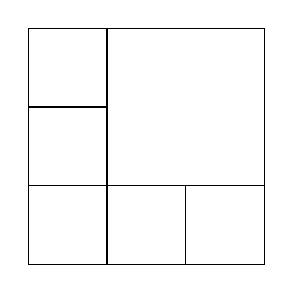
\begin{tikzpicture}
\draw (0,0) -- (3,0) -- (3,3) -- (0,3) -- (0,0);
\draw (1,0) -- (1,3);
\draw (2,0) -- (2,1);
\draw (0,2) -- (1,2);
\draw (0,1) -- (3,1);
\end{tikzpicture}
\end{center}
Having a solution for $n=6$ one can provide solutions for $n=9,12,\ldots$
\begin{center}
\begin{tabular}{ccc}
$n=6$ & $n=9$ & $n=12$\\
 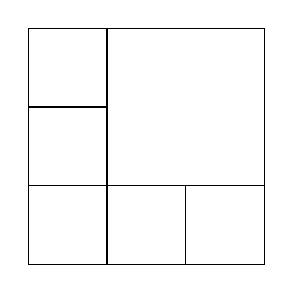
\begin{tikzpicture}
\draw (0,0) -- (3,0) -- (3,3) -- (0,3) -- (0,0);
\draw (1,0) -- (1,3);
\draw (2,0) -- (2,1);
\draw (0,2) -- (1,2);
\draw (0,1) -- (3,1);
\end{tikzpicture}
 &  
 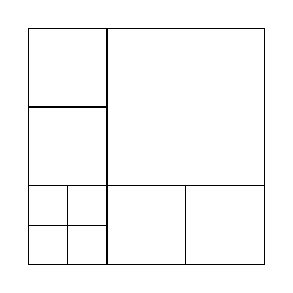
\begin{tikzpicture}
\draw (0,0) -- (3,0) -- (3,3) -- (0,3) -- (0,0);
\draw (1,0) -- (1,3);
\draw (2,0) -- (2,1);
\draw (0,2) -- (1,2);
\draw (0,1) -- (3,1);
\draw (0.5,0) -- (0.5,1);
\draw (0,0.5) -- (1,0.5);
\end{tikzpicture}
 & 
 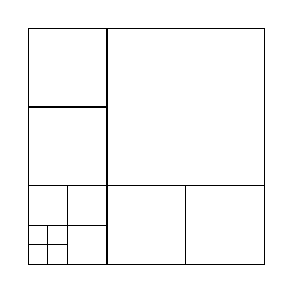
\begin{tikzpicture}
\draw (0,0) -- (3,0) -- (3,3) -- (0,3) -- (0,0);
\draw (1,0) -- (1,3);
\draw (2,0) -- (2,1);
\draw (0,2) -- (1,2);
\draw (0,1) -- (3,1);
\draw (0.5,0) -- (0.5,1);
\draw (0,0.5) -- (1,0.5);
\draw (0,0.25) -- (0.5,0.25);
\draw (0.25,0) -- (0.25,0.5);
\end{tikzpicture}
\end{tabular}
\end{center}
This process works in general, if we have a solution for some $n$, then by subdividing a square into 4 squares
we obtain a solution for $n+3$. We have an argument for part $(b)$ in Mathematical Induction III., namely
with $n_0=3$. If $S(k-2),S(k-1),S(k)$ is true, then $S(k+1)$ is true (since it follows from $S(k-2)$ in this case).
It remains to deal with part $(a)$, that is, we have to show that $S(6),S(7)$ and $S(8)$ are true. We have considered
the case $n=6$. Let us find a solution for $n=7$. We note that the case $n=4$ is easy since 4 is a square. The process
we described allows us to construct a solution for $n=4+3=7$.
\begin{center}
\begin{tabular}{cc}
$n=4$ & $n=7$\\
\begin{tikzpicture}
\draw (0,0) -- (4,0) -- (4,4) -- (0,4) -- (0,0);
\draw (2,0) -- (2,4);
\draw (0,2) -- (4,2);
\end{tikzpicture}
 & 
\begin{tikzpicture}
\draw (0,0) -- (4,0) -- (4,4) -- (0,4) -- (0,0);
\draw (2,0) -- (2,4);
\draw (0,2) -- (4,2);
\draw (1,0) -- (1,2);
\draw (0,1) -- (2,1);
\end{tikzpicture}
\end{tabular}
\end{center}
Finally we handle the remaining case, that is, $n=8$. Here we have the solution: 
\begin{center}
\begin{tikzpicture}
\draw (0,0) -- (4,0) -- (4,4) -- (0,4) -- (0,0);
\draw (1,0) -- (1,4);
\draw (0,1) -- (4,1);
\draw (2,0) -- (2,1);
\draw (3,0) -- (3,1);
\draw (0,2) -- (1,2);
\draw (0,3) -- (1,3);
\end{tikzpicture}
\end{center}


\begin{exercise}\label{induction-1}
Prove that $9^n-1$ is divisible by 8 for all $n\in\mathbb{N}$. 
\end{exercise}

\begin{exercise}\label{induction-2}
Prove that $5^{2n-1}+1$ is divisible by 6 for all $n\in\mathbb{N}$. 
\end{exercise}

\begin{exercise}\label{induction-3}
Prove the following identity by induction
$$
\sum_{i=1}^n (2i-1)=n^2.
$$
\end{exercise}

\begin{exercise}\label{induction-4}
Prove the following identity by induction
$$
\sum_{i=1}^n i^2=\frac{n(n+1)(2n+1)}{6}.
$$
\end{exercise}

\begin{exercise}\label{induction-4a}
Prove the following identity by induction
$$
\sum_{i=1}^n i^3=\left(\frac{n(n+1)}{2}\right)^2.
$$
\end{exercise}

\begin{exercise}\label{ex:sumk(k+1)}
Prove the following identity by induction
\[
\sum_{i=1}^{n-1} {i(i+1)}=\frac{\left(n-1\right)n\left(n+1\right)}{3}.
\]
\end{exercise}

\begin{exercise}\label{induction-4b}
Prove the following identity by induction
$$
\sum_{i=1}^n\frac{1}{i(i+1)}=\frac{n}{n+1}.
$$
\end{exercise}

\begin{exercise}\label{induction-5}
Let $\halmaz{a_n}$ be a sequence defined by
\begin{align*}
a_1&=1,\\
a_2&=8,\\
a_n&=a_{n-1}+2a_{n-2},\quad n\geq 3.
\end{align*}
Prove that
$$
a_n=\frac{3}{2}\cdot 2^n+2 \cdot (-1)^n.
$$
\end{exercise}

\begin{exercise}\label{induction-6}
Prove by induction that the number 
$$
\left(\frac{3-\sqrt{33}}{2}\right)^n+\left(\frac{3+\sqrt{33}}{2}\right)^n
$$
is an integer which is divisible by 3 for all $n\in\mathbb{N}$.
\end{exercise}

\begin{exercise}\label{induction-7}
Let $\halmaz{a_n}$ be a sequence defined by 
\begin{align*}
a_1&=\sqrt{2},\\
a_n&=\sqrt{2+a_{n-1}}\quad n\geq 2.
\end{align*}
Prove by induction that $a_n\leq 2$ for all $n\geq 1$.
\end{exercise}

\begin{exercise}\label{induction-8}
Prove that for all $n\in\mathbb{N}$ there exists an $n$-digit integer
$$
a_1a_2\ldots a_n
$$
whose digits are either 1 or 2 and it is divisible by $2^n$.
\end{exercise}

\begin{exercise}\label{induction-9}
Let $F_n$ be a sequence defined by $F_1=F_2=1$ and $F_n=F_{n-1}+F_{n-2}, n\geq 3$ (this sequence is the so-called Fibonacci sequence).
Prove by induction the following identities.

(a) $F_1+F_2+\ldots+F_n=F_{n+2}-1$,

(b) $F_1^2+F_2^2+\ldots+F_n^2=F_nF_{n+1}$,

(c) $F_1+F_3+\ldots+F_{2n-1}=F_{2n}$,

(d) $F_2+F_4+\ldots+F_{2n}=F_{2n+1}-1$.
\end{exercise}

\begin{exercise}\label{induction-10}
Prove the following properties of Fibonacci numbers.

(a) Prove that $F_{3n}$ is even for all $n\in\mathbb{N}$.  

(b) Prove that $F_{5n}$ is divisible by 5 for all $n\in\mathbb{N}$. 

\end{exercise}



\section{Proofs by contradiction}
In this section we study an important tool to prove mathematical theorems. This tool is called proof by contradiction or
indirect proof. There is a simple logic behind, instead of proving that something must be true, we prove it indirectly by showing 
that it cannot be false. We assume that the opposite of our theorem is true. From this assumption we try to obtain such a conclusion 
which is known to be false. This contradiction then shows that our theorem must be true.

Let us consider a basic example. We try to prove that $\sqrt{2}$ is irrational. We provide an indirect proof. We assume the opposite
of our statement, that is, that $\sqrt{2}$ is rational. Rational numbers can be written as $\frac{a}{b}$ for some $a\in\mathbb{Z}$
and $b\in\mathbb{N}$ such that the greatest common divisor of $a$ and $b$ is 1. So we have 
$$
\sqrt{2}=\frac{a}{b}.
$$
Hence $a^2=2b^2$. It follows that 2 divides $a$, so $a=2a_1$ for some $a_1\in\mathbb{Z}$. We substitute this into the equation
$a^2=2b^2$ and we get $4a_1^2=2b^2$. After dividing by 2 we get $2a_1^2=b^2$. So we have that 2 divides $b$. We have a contradiction
since the greatest common divisor of $a$ and $b$ should be 1, but we obtained that 2 divides $a$ and also divides $b$. Hence 2 divides 
the greatest common divisor. This contradiction shows that our statement must be true, that is, $\sqrt{2}$ is irrational.

In Section \ref{Euc} there is a statement about the Division algorithm which says that given two integers $a$ and $b$ such that $b>0$, 
there exist unique integers $q$ and $r$ for which 
$$
a=qb+r,\quad 0\leq r<b.
$$
Now we prove that $q$ and $r$ are unique. We give a proof by contradiction. Assume that there exist integers $q,q'$ and $r,r'$ such that
$q\neq q'$ or $r\neq r'$ and 
\begin{align*}
a&=qb+r,\quad 0\leq r<b,\\
a&=q'b+r',\quad 0\leq r'<b.
\end{align*}
The above equations imply that 
$$
b(q-q')=r'-r.
$$
It follows that $b$ divides $r'-r$. We also have the inequalities
\begin{align*}
0\leq &r<b,\\
0\leq &r'<b.
\end{align*}
So we have that 
$$
-b<r'-r<b.
$$
There is only one integer in this interval which is a multiple of $b$, namely 0. We obtained that $r'-r=0$, that is, $r'=r$.
Also we have that $b(q-q')=r'-r=0$. Since $b>0$, it is clear that $q-q'=0$ must hold, hence $q=q'$. A contradiction, since we 
assumed that $q\neq q'$ or $r\neq r'$.

Let us consider a proposition about prime numbers (a positive integer is prime if it is greater than 1 and has no positive divisors other than 1 and the number itself.)
If $p,q$ and $r$ are prime numbers, then 
$$
p^2+q^2\neq r^2.
$$
Assume the opposite, that is, there exist prime numbers $p,q$ and $r$ such that $p^2+q^2=r^2$. There are three possibilities
\begin{enumerate}
\item[(1)] $p$ and $q$ are odd primes,
\item[(2)] $p$ and $q$ are even primes,
\item[(3)] one of the primes $p,q$ is even the other is odd.
\end{enumerate}

(1) We have that $p$ and $q$ are odd primes, hence $p^2+q^2=r^2$ is even. If $r^2$ is even, then $r$ is even.
The only even prime number is 2, so we have $r=2$. That is, $p^2+q^2=4$. Since $p$ and $q$ are odd primes we have $p,q\geq 3$.
Therefore $p^2+q^2\geq 18$, a contradiction. We proved that if $p$ and $q$ are odd primes, then the statement must be true.

(2) We have that $p$ and $q$ are even primes, that is, $p=q=2$. We obtain that $8=r^2$. It implies that $r$ is even, so $r=2$.
A contradiction since $r^2=4$ while we concluded that $r^2$ must be 8. In this case our statement turns out to be true.

(3) We may suppose that $p$ is even and $q$ is odd. That is, $p=2$ and $q=2q_1+1$ for some $q_1$. It is clear that $r$ is also odd,
since its square is a sum of an even number and an odd number, that is, $r=2r_1+1$. Our equation implies that
$4+(2q_1+1)^2=(2r_1+1)^2$, which can be written as
$$
4+4q_1^2+4q_1+1=4r_1^2+4r_1+1.
$$
One gets that
$$
q_1(q_1+1)+1=r_1(r_1+1).
$$
The product of two consecutive integers is even, so $q_1(q_1+1)$ and $r_1(r_1+1)$ are even. Then we have that $r_1(r_1+1)-q_1(q_1+1)$
is an even integer, but the above equation implies that 
$$
r_1(r_1+1)-q_1(q_1+1)=1,
$$
a contradiction since 1 is not an even integer.

Now we prove a result related to prime numbers. The proof we provide is a nice indirect proof due to Euclid.
\begin{proposition}
There are infinitely many prime numbers.
\end{proposition}
\begin{proof}
Suppose that there are only finitely many primes, let say $p_1<p_2<p_3<\ldots<p_n$. Let us consider the integer
$$
N=p_1p_2\cdots p_n+1.
$$
Since $N$ is not on the list of prime numbers it must have a prime divisor. It means that for some $1\leq i\leq n$
the prime $p_i$ divides $N$. Applying the Division algorithm we obtain
$$
N=\left(\prod_{1\leq k\leq n, k\neq i}p_k\right)\cdot p_i+1,
$$
that is, the remainder is equal to 1. Thus $N$ is not divisible by $p_i$, a contradiction. Thus we have proved
that there are infinitely many primes.
\end{proof}

\begin{exercise}\label{contra-0}
Prove that if $x+y>10$ for some $x,y\in\mathbb{Z}$, then $x>5$ or $y>5$. 
\end{exercise}

\begin{exercise}\label{contra-0a}
Prove that there exists no integer $n$ such that $n^2-2$ is a multiple of 4.
\end{exercise}

\begin{exercise}\label{contra-1}
Prove that $\sqrt{2}+\sqrt{3}$ is irrational.
\end{exercise}

\begin{exercise}\label{contra-2}
Prove that if $a,b$ and $c$ are odd integers, then the equation
$$
ax^2+bx+c=0
$$
has no solution with $x\in\mathbb{Q}$.
\end{exercise}

\begin{exercise}\label{contra-3}
Given $n$ integers $a_1,a_2,\ldots,a_n$, prove that there exists $1\leq i\leq n$
such that
$$
a_i\geq \frac{a_1+a_2+\ldots+a_n}{n}.
$$
\end{exercise}

\begin{exercise}\label{contra-4}
Let $F_n$ be a sequence defined by $F_1=F_2=1$ and $F_n=F_{n-1}+F_{n-2}, n\geq 3$, that is, the Fibonacci sequence.
Prove that $\gcd(F_n,F_{n+1})=1$ for all positive integer $n$.
\end{exercise}



\section{Constructive proofs}
In this section we deal with several problems for which a method can be provided to create a solution.
We consider the coin problem (known also as the Frobenius problem). Let us be given a currency system with
$k\geq 2$ distinct integer denominations $a_1<a_2<\ldots<a_k$. Which amounts can be changed? This question
yields the following linear Diophantine equation
$$
a_1x_1+a_2x_2+\ldots+a_kx_k=n,
$$
where $x_1,\ldots,x_k$ are non-negative integers. Now we study the case $k=2$, that is, our equation is
$$
a_1x_1+a_2x_2=n.
$$
There are some natural questions to pose:
\begin{itemize}
\item
Does the equation possess integer solutions?
\item
How many solutions does it have?
\item
How to determine all solutions?
\end{itemize}

In what follows we consider the above problem but we allow integer solutions instead of non-negative integer 
solutions. We will use these results to answer the original question.

Assume that $\gcd(a_1,a_2)=d$. Since $d$ divides $a_1x_1+a_2x_2$ we easily get that $d$ divides $n$,
if there is a solution in integers. For example, if we consider the equation
$$
6x_1+8x_2=5,
$$
then 2 divides $6x_1+8x_2$, but 2 does not divide 5. Therefore there is no solution in integers.

Now suppose that $(u_1,u_2)$ is a solution, that is, $a_1u_1+a_2u_2=n$. Assume that there exists a
different solution, say $(v_1,v_2)$. We have that
\begin{align*}
a_1u_1+a_2u_2&=n,\\
a_1v_1+a_2v_2&=n.
\end{align*}
It implies that
$$
a_1(u_1-v_1)=a_2(v_2-u_2).
$$
Let $b_1=a_1/d$ and $b_2=a_2/d$. Since $d$ is the largest common divisor of $a_1$ and $a_2$, 
we obtain that $\gcd(b_1,b_2)=1$. We simplify the above equation by $d$ to get
$$
b_1(u_1-v_1)=b_2(v_2-u_2).
$$
It is clear that $b_1$ divides $v_2-u_2$, since $\gcd(b_1,b_2)=1$. So we have $v_2-u_2=b_1t$ 
for some $t\in\mathbb{Z}$. Thus 
$$
v_2=u_2+b_1t,
$$
and
$$
v_1=u_1-b_2t.
$$
It follows that there are infinitely many integer solutions. We have proved that there is no solution if 
$\gcd(a_1,a_2)$ does not divide $n$, and if there is a solution, then there are infinitely many integer solutions.
In Section \ref{Euc} we showed that one can use the Euclidean algorithm to determine integers $x,y$ for which
$a_1x+a_2y=\gcd(a_1,a_2)=d$. Now assume that $d$ divides $n$, that is, $n=n_1d$ for some $n_1$. We obtain the following 
equation
$$
a_1xn_1+a_2yn_1=dn_1=n.
$$
Therefore $(xn_1,yn_1)$ is a solution of the equation $a_1x_1+a_2x_2=n$. Let us summarize what we obtained.
\begin{theorem}\label{LinDioph}
 Let $a_1,a_2$ and $n$ be integers with $a_1$ and $a_2$ not both zero.
 The linear Diophantine equation $a_1x_1+a_2x_2=n$ has a solution if and only if $\gcd(a_1,a_2)$ divides $n$.
 
 If $\gcd(a_1,a_2)$ divides $n$ and $(x,y)$ is a solution of the equation $a_1x+a_2y=\gcd(a_1,a_2)$ provided
 by the Euclidean algorithm, then
 $$
 \left(\frac{xn}{\gcd(a_1,a_2)},\frac{yn}{\gcd(a_1,a_2)}\right)
 $$
 is a solution of the equation $a_1x_1+a_2x_2=n$.

 If $(u_1,u_2)$ is a solution of the equation $a_1x_1+a_2x_2=n$, then
$$
\left(u_1-\frac{a_2}{\gcd(a_1,a_2)}t, u_2+\frac{a_1}{\gcd(a_1,a_2)}t\right),\quad t\in\mathbb{Z}
$$
are solutions of the equation $a_1x_1+a_2x_2=n$.
\end{theorem}
We apply the previous method to determine all integer solutions of the equation
$$
132x_1+187x_2=55.
$$
First we find the greatest common divisor of 132 and 187. We use the Euclidean algorithm:
\begin{align*}
187 &= 1\cdot 132+55\\
 132 &= 2\cdot 55+22\\
 55 &= 2\cdot 22 + 11\\
 22 &= 2\cdot 11 + 0.
\end{align*}
That is, $\gcd(132,187)=11$. Since 11 divides 55 we know that there are infinitely many integer solutions.
The next step is to construct a solution to the equation $132x+187y=11:$
\begin{align*}
11&= 55-2\cdot 22\\
  &= 55-2\cdot (132-2\cdot 55)=-2\cdot 132+5\cdot 55\\
  &= -2\cdot 132+5\cdot (187-132)=5\cdot 187-7\cdot 132.
\end{align*}
We obtained that $x=-7, y=5$ is a solution to the equation $132x+187y=11$.
Hence we have
$$
132\cdot (-7\cdot 5)+187\cdot (5\cdot 5)=55.
$$
It implies that $x_1=-35,x_2=25$ is a solution to the equation $132x_1+187x_2=55$. Our theorem yields that
$$
\left(-35-17t, 25+12t\right)\quad t\in\mathbb{Z}
$$
are solutions of the equation $132x_1+187x_2=55$.

We can handle equations of the form $a_1x_1+a_2x_2=n$ in $x_1,x_2\in\mathbb{Z}$. If we have $\gcd(a_1,a_2)=1$,
then we can solve the equation for any $n$ in integers. What can we say about this equation if we allow only
non-negative integers? Let us deal with the equation $$7x_1+11x_2=n.$$ From the Euclidean algorithm we get that
$$
7\cdot(-3)+11\cdot 2=1.
$$
Thus we have that
$$
(-3n,2n)
$$
is a solution to the equation $7x_1+11x_2=n$. From this particular solution we get infinitely many solutions:
$$
(-3n-11t,2n+7t)\quad t\in\mathbb{Z}.
$$
We would like to have non-negative solutions, hence
\begin{align*}
-3n-11t&\geq 0\Rightarrow t\leq \frac{-3n}{11}\\
2n+7t&\geq 0\Rightarrow t\geq \frac{-2n}{7}.
\end{align*}
So we have the following inequalities
$$
\frac{-2n}{7}\leq t\leq \frac{-3n}{11}.
$$
If there is an integer contained in the interval $[\frac{-2n}{7},\frac{-3n}{11}]$, then $n$ can be represented
in the form $7x_1+11x_2$. Denote by $I_n$ the set $\halmazvonal{t}{ \frac{-2n}{7}\leq t\leq \frac{-3n}{11}, t\in\mathbb{Z}}$.
\begin{center}
\begin{tabular}{|c|c||c|c||c|c||c|c||c|c|}
\hline
$n$ & $I_n$ & $n$ & $I_n$ & $n$ & $I_n$ & $n$ &  $I_n$ & $n$ & $I_n$ \\
\hline
1 & $\emptyset$ & 16 & $\emptyset$ & 31 & $\emptyset$ & 46 & $\halmaz{-13}$ & 61 & $\halmaz{-17}$\\
\hline
2 & $\emptyset$ & 17 & $\emptyset$ & 32 & $\halmaz{-9}$ & 47 & $\halmaz{-13}$ & 62 & $\halmaz{-17}$\\
\hline
3 & $\emptyset$ & 18 & $\halmaz{-5}$ & 33 & $\halmaz{-9}$ & 48 & $\emptyset$ & 63 & $\halmaz{-18}$\\
\hline
4 & $\emptyset$ & 19 & $\emptyset$ & 34 & $\emptyset$ & 49 & $\halmaz{-14}$ & 64 & $\halmaz{-18}$\\
\hline
5 & $\emptyset$ & 20 & $\emptyset$ & 35 & $\halmaz{-10}$ & 50 & $\halmaz{-14}$ & 65 & $\halmaz{-18}$\\
\hline
6 & $\emptyset$ & 21 & $\halmaz{-6}$ & 36 & $\halmaz{-10}$ & 51 & $\halmaz{-14}$ & 66 & $\halmaz{-18}$\\
\hline
7 & $\halmaz{-2}$ & 22 & $\halmaz{-6}$ & 37 & $\emptyset$ & 52 & $\emptyset$ & 67 & $\halmaz{-19}$\\
\hline
8 & $\emptyset$ & 23 & $\emptyset$ & 38 & $\emptyset$ & 53 & $\halmaz{-15}$ & 68 & $\halmaz{-19}$\\
\hline
9 & $\emptyset$ & 24 & $\emptyset$ & 39 & $\halmaz{-11}$ & 54 & $\halmaz{-15}$ & 69 & $\halmaz{-19}$\\
\hline
10 & $\emptyset$ &25 & $\halmaz{-7}$ &40  & $\halmaz{-11}$ &55  & $\halmaz{-15}$ &70  & $\halmaz{-20}$\\
\hline
11 & $\halmaz{-3}$ &26  & $\emptyset$ &41  & $\emptyset$ &56  & $\halmaz{-16}$ &71  & $\halmaz{-20}$\\
\hline
12 & $\emptyset$ &27  & $\emptyset$ &42  & $\halmaz{-12}$ &57  & $\halmaz{-16}$ &72  & $\halmaz{-20}$\\
\hline
13 & $\emptyset$ &28  & $\halmaz{-8}$ &43  & $\halmaz{-12}$ &58  & $\halmaz{-16}$ &73  & $\halmaz{-20}$\\
\hline
14 & $\halmaz{-4}$ &29  & $\halmaz{-8}$ &44  & $\halmaz{-12}$ &59  & $\emptyset$ &74  & $\halmaz{-21}$\\
\hline
15 & $\emptyset$ &30  & $\emptyset$ &45  & $\emptyset$ &60  & $\halmaz{-17}$ &75  & $\halmaz{-21}$\\
\hline
\end{tabular}
\end{center}
We can find 7 consecutive integers indicated in the table for which the set $I_n$ is not empty,
that is, those integers can be represented in the form $7x_1+11x_2:$
\begin{align*}
n&=60 & x_1=(-3)\cdot 60-11\cdot(-17)=7, x_2=2\cdot 60+7\cdot(-17)=1,\\
n&=61 & x_1=(-3)\cdot 61-11\cdot(-17)=4, x_2=2\cdot 61+7\cdot(-17)=3,\\
n&=62 & x_1=(-3)\cdot 62-11\cdot(-17)=1, x_2=2\cdot 62+7\cdot(-17)=5,\\
n&=63 & x_1=(-3)\cdot 63-11\cdot(-18)=9, x_2=2\cdot 63+7\cdot(-18)=0,\\
n&=64 & x_1=(-3)\cdot 64-11\cdot(-18)=6, x_2=2\cdot 64+7\cdot(-18)=2,\\
n&=65 & x_1=(-3)\cdot 65-11\cdot(-18)=3, x_2=2\cdot 65+7\cdot(-18)=4,\\
n&=66 & x_1=(-3)\cdot 66-11\cdot(-18)=0, x_2=2\cdot 66+7\cdot(-18)=6.
\end{align*}
Given a solution for $n=60$ we can easily find a solution for $n=67$ and $n=74$ etc. We use this idea to
provide solutions for all $n>59$. The Division algorithm says that if we divide an integer by 7, then the 
remainder is between 0 and 6. 

If the remainder is 0, then from the equation $63=7\cdot 9+11\cdot 0$ we get
$$
7(k+9)=7(k+9)+11\cdot 0,\quad k\geq 0.
$$
That is, if we have an integer $n\geq 63$ divisible by 7, then it can be written in the form $7x_1+11x_2$ with $x_1,x_2\geq 0$.

If the remainder is 1, then we use the equation $64=7\cdot 6+11\cdot 2$ to obtain
$$
7(k+9)+1=7(k+6)+11\cdot 2,\quad k\geq 0.
$$
In a similar way one computes the general solutions for the remaining cases.

How to deal with equations with more than two variables? We show how to reduce equations in three unknowns to
equations in two unknowns. So the techniques applied previously can be used here. Consider the equation
$$
4x_1+5x_2+7x_3=n,\quad x_1,x_2,x_3\in\mathbb{Z}.
$$
Introduce a new variable $y_1=4x_1+5x_2$, then the equation can be written as
$$
y_1+7x_3=n.
$$
A particular solution is $(n,0)$, hence all the integer solutions can be parametrized as follows
\begin{align*}
y_1&=n+7t,\\
x_3&=-t,
\end{align*}
for some $t\in\mathbb{Z}$. It remains to determine the integer solutions of the equation $y_1=4x_1+5x_2=n+7t$.
The first thing to do is to find a particular solution. It is easy to check that
\begin{align*}
x_1&=-n+3t,\\
x_2&=n-t\\
\end{align*}
is a solution. Applying the techniques used in case of two variables we get the following parametrization of
integral solution
\begin{align*}
x_1&=-n+3t-5s,\\
x_2&=n-t+4s,\\
x_3&=-t
\end{align*}
for some $s,t\in\mathbb{Z}$. As a concrete example consider the equation $4x_1+5x_2+7x_3=23$. Then we obtain
integer solutions by substituting concrete integral values into the above formulas. Some solutions are indicated
in the following table
\begin{center}
\begin{tabular}{|c|c|}
\hline
$(s,t)$ & $(x_1,x_2,x_3)$\\
\hline
$(0,0)$ & $(-23, 23, 0)$\\
\hline
$(-1,0)$ & $(-18, 19, 0)$\\
\hline
$(0,-1)$ & $(-26, 24, 1)$\\
\hline
$(1,0)$ & $(-28, 27, 0)$\\
\hline
$(0,1)$ & $(-20, 22, -1)$\\
\hline
$(-1,-1)$ & $(-21, 20, 1)$\\
\hline
$(1,1)$ & $(-25, 26, -1)$\\
\hline
\end{tabular}
\end{center}

What about non-negative integer solutions? That is, if one asks for solutions such that $x_1,x_2,x_3\in\mathbb{N}\cup\halmaz{0}$.
In case of the equation $4x_1+5x_2+7x_3=n$ we determined the parametrization of the integral solutions, so we get the
following inequalities
\begin{align*}
0&\leq -n+3t-5s,\\
0&\leq n-t+4s,\\
0&\leq -t.
\end{align*}
That is, we immediately see that $t\leq 0$. We try to eliminate $s$ from the first and the second equations. So we multiply by 4 the first equation
and by 5 the second one and we get
$$
5t-5n\leq 20s\leq -4n+12t.
$$
That is, we obtain that
$$
-\frac{n}{7}\leq t\leq 0.
$$
It remains to determine a lower bound and an upper bound for $s$. We have
$$
20s\geq 5t-5n\geq -5\frac{n}{7}-5n,
$$
hence $s\geq -\frac{2n}{7}$. Similarly, we have
$$
20s\leq -4n+12t\leq -4n,
$$
therefore $s\leq -\frac{n}{5}$. Let us denote the two intervals as $I_s=[-\frac{2n}{7},-\frac{n}{5}]$ and $I_t=[-\frac{n}{7},0]$.
To have a non-negative integer solution we need an integer contained in the interval $I_s$ and another one contained in $I_t$.
If the length of the interval $I_s$ is at least 1 and similarly for $I_t$, then for sure there will be such integers.
The length of $I_s$ is $-\frac{n}{5}+\frac{2n}{7}=\frac{3n}{35}$ and the length of $I_t$ is $\frac{n}{7}$. We have that the length
of $I_s$ is at least 1 if $n\geq 12$ and the length of $I_t$ is at least 1 if $n\geq 7$. If $n\geq 12$, then an integer solution
is guaranteed. It means that if $n\geq 12$, then the equation $4x_1+5x_2+7x_3=n$ has non-negative integer solution. Now we deal with
the remaining cases $1\leq n\leq 11.$
\begin{center}
\begin{tabular}{|c|c|c|c|}
\hline
$n$ & integer(s) in $I_s$ & integer(s) in $I_t$ & solution(s): $(x_1,x_2,x_3)$\\
\hline
1 &- & 0 & -\\
\hline
2 &- & 0 & -\\
\hline
3 &- & 0 & -\\
\hline
4 &-1 & 0 & $(1,0,0)$\\
\hline
5 &-1 & 0 & $(0,1,0)$\\
\hline
6 &- & 0 & -\\
\hline
7 &-2 &-1,0 & $(0,0,1)$\\
\hline
8 &-2 & -1,0 & $(2,0,0)$\\
\hline
9 &-2 &-1,0  & $(1,1,0)$\\
\hline
10&-2 &-1,0  & $(0,2,0)$\\
\hline
11&-3 &-1,0  & $(1,0,1)$\\
\hline
\end{tabular}
\end{center}
We proved that if $n>6$, then the equation $4x_1+5x_2+7x_3=n$ has non-negative integer solution.


\begin{exercise}\label{proof-cons-1}
Prove that all integers $n\geq 24$ can be written as $5x_1+7x_2$ for some non-negative integers $x_1,x_2$.
\end{exercise}

\begin{exercise}\label{proof-cons-2}
Prove that all integers $n\geq 12$ can be written as $4x_1+5x_2$ for some non-negative integers $x_1,x_2$.
Determine a formula for the solution in case of integers of the form $n=4K+1$.
\end{exercise}

\begin{exercise}\label{proof-cons-3}
Parametrize all integer solutions of the equation
$$
4x_1+6x_2+9x_3=n.
$$
\end{exercise}

\begin{exercise}\label{proof-cons-4}
Determine the largest positive integer $n$ for which the equation 
$$
4x_1+6x_2+9x_3=n
$$
has no non-negative integer solution.
\end{exercise}


\section{Pigeonhole principle}
In this section we study the so-called pigeonhole principle which is a simple tool to prove several interesting results.
First we prove the simplest form of the pigeonhole principle.
\begin{theorem}
If $n+1$ pigeons are placed into $n$ pigeonholes, then there exists a pigeonhole containing at least 2 pigeons.
\end{theorem}
\begin{proof}
Assume that the statement is false. That is, each pigeonhole contains at most one pigeon. In this case the total number of 
pigeons is at most $n$, a contradiction.
\end{proof}
One can easily generalize the above theorem. We have the following.
\begin{theorem}
If $mn+1$ pigeons are placed into $n$ pigeonholes, then there exists a pigeonhole containing at least $m+1$ pigeons.
\end{theorem}
\begin{proof}
Again we prove the statement by contradiction. Assume that the statement is false, that is, each pigeonhole contains at most $m$ pigeons.
We obtain that the total number of pigeons is at most $mn$, a contradiction since there are $mn+1$ pigeons.
\end{proof}
Finally we prove a version where the pigeonholes may contain different number of pigeons.
\begin{theorem}\label{pigeon-III}
Let $m_1,m_2,\ldots,m_n$ are positive integers. If $m_1+m_2+\ldots+m_n-n+1$ pigeons are placed into $n$ pigeonholes, then for some
$1\leq i\leq n$ one has that the $i$th pigeonhole contains at least $m_i$ pigeons.
\end{theorem}
\begin{proof}
Suppose that the first pigeonhole contains at most $m_1-1$ pigeons, the second contains at most $m_2-1$ pigeons etc., the 
$n$th pigeonhole contains at most $m_n-1$ pigeons. The total number of pigeons contained in the $n$ pigeonholes can be at most
$$
(m_1-1)+(m_2-1)+\ldots+(m_n-1)=m_1+m_2+\ldots+m_n-n,
$$
a contradiction since there are $m_1+m_2+\ldots+m_n-n+1$ pigeons.
\end{proof}

To apply the pigeonhole principle one has to decide what the pigeons are. Then one has to identify the pigeonholes in such a way
that if two pigeons are in the same pigeonhole, then they have some special property in common. It is important that we need more
pigeons than pigeonholes. In what follows we solve several concrete problems by using the pigeonhole principle.
\begin{proposition}
There is a nonzero multiple of 6 whose digits are all zeroes and ones. 
\end{proposition}
\begin{proof}
We apply the pigeonhole principle and the Division algorithm. Consider the integers $a_n=\sum_{k=0}^n 10^k$ for $n=0,1,2,3,4,5$.
We can write these numbers as $q_n\cdot 6+r_n$, where $q_n$ is the quotient and $r_n$ is the remainder, so $0\leq r_n<6$. There are six
possibilities for $r_n$ and there are six integers $a_0,a_1,\ldots,a_5$. The numbers $a_0,a_1,\ldots,a_5$ are odd integers while 6 is even,
hence $r_n\neq 0$ for all $n$. We have that $r_n\in\halmaz{1,2,3,4,5}$ for all $n$. There are only 5 pigeonholes (possible remainders) and 6 pigeons (integers $a_n$).
We obtain that there are at least two integers having the same remainder, say, $a_{m_1}$ and $a_{m_2}$, where $m_1<m_2$. In this case $a_{m_2}-a_{m_1}$ is
divisible by 6 and all the digits are zeroes and ones.
\begin{center}
\begin{tabular}{|c|c|c|}
\hline
$n$ & $a_n$ & $q_n\cdot 6+r_n$\\
\hline
0 & 1&$0\cdot 6+1$\\
\hline
1 &11& $1\cdot 6+5$\\
\hline
2 &111&$18\cdot 6+3$\\
\hline
3 &1111&$185\cdot 6+1$\\
\hline
4 &11111&$1851\cdot 6+5$\\
\hline
5 & 111111 & $18518\cdot 6+3$\\
\hline
\end{tabular}
\end{center}
It is clear that $r_0=r_3=1$, therefore $a_3-a_0=1111-1=1110$ is a multiple of 6 ($1110=185\cdot 6$) and this integer is in a right form.
\end{proof} 

\begin{proposition}
Let $A$ be a set containing $n\geq 2$ integers. There is a subset of $A$ such that the sum of its elements is a 
multiple of $n$.
\end{proposition}
\begin{proof}
We have a set containing $n$ elements, let us say these are $a_1,a_2,\ldots,a_n$. We define $n$ subsets as follows
$$
S_k=\halmaz{a_1,\ldots,a_k},\quad k=1,2,\ldots,n,
$$
that is, $S_1=\halmaz{a_1}, S_2=\halmaz{a_1,a_2},\ldots,S_n=A$. Denote by $s_k$ the sum of the elements of $S_k$. We apply the
Division algorithm to write $s_k=q_k\cdot n+r_k$, where $0\leq r_k<n$. If for some $k$ we have $r_k=0$, then
$$
s_k=a_1+\ldots+a_k=q_k\cdot n,
$$
that is, the sum of the elements of $S_k$ is a multiple of $n$. In this case the theorem is true. If no such
$k$ exists, then we have only $n-1$ possible values for $r_k$ and we have $n$ subsets. The pigeonhole principle says
that there are at least two subsets (say $S_k$ and $S_l, k<l$) for which $r_k=r_l$. In this case we obtain that
$$
s_l-s_k=(q_l-q_k)n=a_{k+1}+a_{k+2}+\ldots+a_l.
$$
Thus the sum of the elements of the subset $\halmaz{a_{k+1},a_{k+2},\ldots,a_l}$ is a multiple of $n$.
\end{proof}

\begin{exercise}\label{pigeon-0a}
Prove that among 367 people, at least two were born on the same day of the year.
\end{exercise}

\begin{exercise}\label{pigeon-0b}
Prove that among 1500 people, at least four were born on the same day of the year.
\end{exercise}


\begin{exercise}\label{pigeon-1}
Prove that if seven distinct integers are selected from the set $$\halmaz{1,2,3,4,5,6,7,8,9,10,11,12},$$
then two of these integers sum to 13.
\end{exercise}

\begin{exercise}\label{pigeon-2}
We choose 11 integers from the set $\halmaz{1,2,\ldots,20}$. Prove that 2 of the chosen
integers are consecutive.
\end{exercise}

\begin{exercise}\label{pigeon-3}
 Prove that if five points are selected from the interior of a unit square, then there are two points whose distance is less than
$\sqrt{2}/2$.
\end{exercise}

\begin{exercise}\label{pigeon-4}
Let $A=\halmaz{1,2,\ldots,100}$. Prove that if we choose 51 distinct integers from $A$, then there are at least two integers
such that one of them is divisible by the other.
\end{exercise}

\begin{exercise}\label{pigeon-5}
How many students in a class must there be to ensure that 4 students get the same grade (one of 1, 2, 3, 4, or 5)?
\end{exercise}

\begin{exercise}\label{pigeon-6}
How many bishops can one place on an $8\times 8$ chessboard such that no two bishops can hit each other?
\end{exercise}

\section{A card trick}
In this section we introduce a card trick, which is based on several mathematical ideas. In fact the trick combines several tools from
this chapter. To understand how it works one should be familiar with the pigeonhole principle, proof by contradiction and some tiny 
amount of combinatorics. Here is the trick. 

An assistant asks the audience to choose five cards from a normal deck of 52 playing cards. They can choose any five as they like.
They pass those five cards to the assistant, who reveals four of them to the magician, one remains only known by the audience and the 
assistant. The magician looks at the four cards handed to him and announces the 5th card, the secret one.

This mathematical card trick was invented by William Fitch Cheney Jr. and it was first published by Wallace Lee in Maths Miracles in 1950.\footnote{William Wallace Lee, \emph{Maths Miracles}, Durham, N.~C. (1950)}

How does this trick work? First we apply the pigeonhole principle to obtain a very important imformation. There are only 4 suits (clubs $\clubsuit$, diamonds $\diamondsuit$, 
hearts $\heartsuit$ and spades $\spadesuit$) while there are 5 cards choosen. An application of pigeonhole principle yields that at least 2 cards must be of the same suit.
The assistant and the magician have an agreement about the ordering of cards, e.g.\ $A-2-3-\ldots-J-Q-K$. There are two cards having the same suit, say $C_1$ and $C_2$. 

\begin{wrapfigure}{r}{0.43\textwidth}
\includegraphics[width=0.4\textwidth]{KartyaKorbe.pdf}
\end{wrapfigure}
It is possible to define a distance between them. One considers the 13 same-suit cards arranged in a circle from $A$ to $K$ going clockwise. 
Given $C_1$ and $C_2$ one defines the distance $d(C_1,C_2)$ as the clockwise distance from $C_1$ to $C_2$. The second observation is that either $d(C_1,C_2)\leq 6$ or $d(C_2,C_1)\leq 6$. This statement can be proved
indirectly. Assume that $d(C_1,C_2)>6$ and $d(C_2,C_1)>6$. Then there must be at least 14 cards having the same suit, a contradiction.
Let us consider an example. 
%(we use the notation $1=A, 11=J, 12=Q, 13=K$).
%\begin{center}
%\tikz[baseline]\node[new polygon={13}{8mm}] {};
%\end{center}
If the two cards are $C_1=3$ and $C_2=J,$ then we have that $d(3,J)=8$ and $d(J,3)=5$. This fact is used to decide which card is going to be at the top of the pile. Assume that $d(C_i,C_j)\leq 6$. The assistant will
place card $C_i$ at the top of the pile and $C_j$ will be the hidden card. The assistant still has to decide how to order the remaining 3 cards. Here comes a tiny combinatorics
involved, three cards can be ordered in $3!=6$ different ways. That is, somehow the assistant will be able to encode the distance $d(C_i,C_j)\leq 6$. The 52 cards are ordered following the 
rules: 

rule I.: $\clubsuit<\diamondsuit<\heartsuit<\spadesuit$,

rule II.: $A<2<3<\ldots<J<Q<K$,

\noindent So we have $A\clubsuit<2\clubsuit<\ldots<Q\spadesuit<K\spadesuit$. Back to the last three cards.
Let us denote by 1 the card having the lowest rank, by 3 the card having the highest rank and by 2 the remaining one.
It is easy to make an agreement about the encoding of the distance, an example is given in the following table
\begin{center}
\begin{tabular}{|c|c|}
\hline
$d(C_i,C_j)$ & order of the 3 cards\\
\hline
1 & 1,2,3\\
\hline
2 & 1,3,2\\
\hline
3 & 2,1,3\\
\hline
4 & 2,3,1\\
\hline
5 & 3,1,2\\
\hline
6 & 3,2,1\\
\hline
\end{tabular}
\end{center}
It is time to start the card trick! Assume that the assistant gets the following cards from the audience: $3\clubsuit, K\clubsuit, 8\diamondsuit, 5\heartsuit$ and $Q\spadesuit$.
Here $3\clubsuit, K\clubsuit$ are two cards having the same suit. What about their distance? One has 
\begin{align*}
d(3\clubsuit, K\clubsuit)&= 10,\\
d(K\clubsuit, 3\clubsuit)&= 3.
\end{align*}
The assistant has to encode 3. The ordering of the remaining three cards is $(1=8\diamondsuit)<(2=5\heartsuit)<(3=Q\spadesuit)$. That is, 
$$
d(K\clubsuit, 3\clubsuit)=3\Rightarrow 5\heartsuit, 8\diamondsuit, Q\spadesuit.
$$
Therefore the pile of cards the assistant gives to the magician is 
$$
K\clubsuit, 5\heartsuit, 8\diamondsuit, Q\spadesuit.
$$

\begin{exercise}\label{card-1}
What card is being encoded by the following sequences of four cards?

(a) $7\clubsuit,3\diamondsuit,J\diamondsuit,A\spadesuit$,

(b) $J\diamondsuit,9\clubsuit,Q\heartsuit,8\heartsuit$,

(c) $9\heartsuit,10\heartsuit,J\diamondsuit,6\diamondsuit$,

(d) $10\diamondsuit,4\spadesuit,2\spadesuit,5\diamondsuit$,

(e) $8\spadesuit,7\diamondsuit,7\heartsuit,3\heartsuit$.
\end{exercise}

\begin{exercise}\label{card-2}
Which card should be the hidden card? How to order the remaining four cards to encode the hidden one?

(a) $3\clubsuit,7\clubsuit,5\diamondsuit,2\diamondsuit,A\spadesuit$,

(b) $10\clubsuit,A\diamondsuit,J\diamondsuit,8\heartsuit,4\spadesuit$,

(c) $A\clubsuit,6\diamondsuit,K\heartsuit,7\spadesuit,8\spadesuit$,

(d) $7\clubsuit,8\diamondsuit,3\spadesuit,7\spadesuit,9\spadesuit$,

(e) $J\diamondsuit,Q\diamondsuit,7\heartsuit,10\heartsuit,3\spadesuit$.
\end{exercise}
